\chapter{Sexual Conduct}

\begin{itemize}
\tightlist
\item
  \textbf{Pr 1,} Sexual intercourse
\item
  \textbf{Sg 1,} Intentional emission of semen
\end{itemize}

\section{Pr 1, Sexual intercourse}

\includemap{../../src/includes/mindmaps/pr-1.png}

\begin{itemize}
\tightlist
\item
  "\ldots{} For \emph{that} action you would only suffer death, for
  \emph{this} action you will suffer in hell.
\item
  As a man with his head cut off cannot become one to live again.
\item
  As a withered leaf separated from its stem cannot be joined again.
\item
  As a flat stone that has been broken in half cannot be put together
  again.
\item
  As a palmyra tree cut off at the crown is incapable of further
  growth."
\end{itemize}

\section{Sg 1, Intentional emission of semen}

\includemap{../../src/includes/mindmaps/sg-1.png}

\begin{itemize}
\tightlist
\item
  ``with the same hand you use to eat the gifts of the faithful''
\item
  trust and good will of the supporters, social contract
\end{itemize}

\subsection{Probation and Penance}

Overview of the procedure after a Sanghadisesa offence, comparing the
case of immediately informing and concealing:

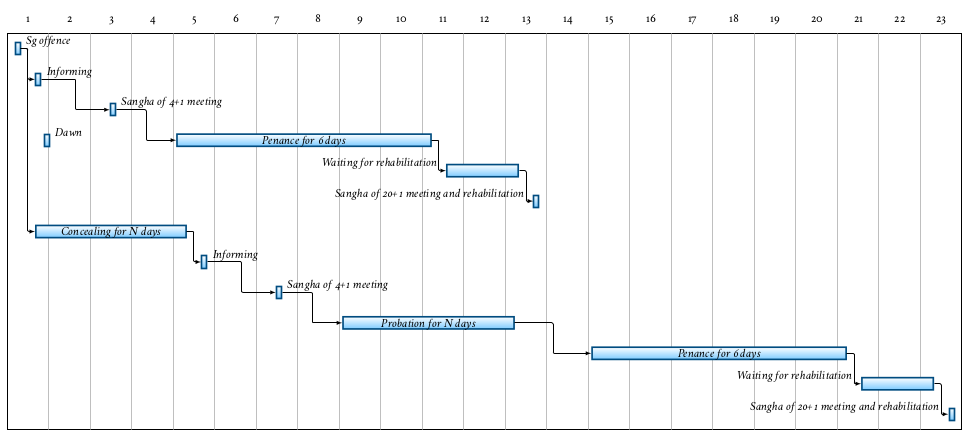
\includegraphics{../../src/includes/figures/sanghadisesa-procedure.png}

One doesn't have to wait until one is certain about the offence,
speaking to another bhikkhu about a doubtful situation will at least
clear one's conscience that one is not concealing it.

A bhikkhu who comitted a sanghadisesa must inform another bhikkhu as
soon as possible, but at most until the next dawnrise. The Sangha must
meet and at his request, allow a six-dawn period of penance
(\emph{mānatta}). If he concealed the offence, a probation period
(\emph{parivāsa}) is required beforehand.

The Sangha will determine when and where the bhikkhu should observe the
\emph{parivāsa} and \emph{mānatta}. These periods are determined by the
Sangha and don't have to occur back-to-back.

After completing \emph{mānatta} he can only be rehabilitated as a
bhikkhu in regular standing by a community meeting of at least 20
bhikkhus. He is not required to stay at that particular monaster after
having received rehabilitation.

If he commits another sanghadisesa before rehabilitation, he must inform
a bhikkhu and ask a Sangha of at least four to `send him back to the
beginning.'

There is allowance to interrupt and set aside the penance or probation
for a period of time, for example when many visiting monks are expected
to arrive at the monastery for an event.

Characteristic duties during penance:

\begin{itemize}
\tightlist
\item
  not receiving duties of respect from other bhikkhus
\item
  inform visiting bhikkhus that he is undergoing penance
\item
  every day, notify every bhikkhu in the monastery of his offence
\item
  stay under a separate roof than the other bhikkhus
\item
  only leave the monastery when accompanied by four other bhikkhus
\end{itemize}

The duties during probation are the same as during penance, except:

\begin{itemize}
\tightlist
\item
  inform the Sangha of his offence every fortnight, not every day
\item
  only leave the monastery when accompanied by a single other bhikkhu
\end{itemize}

\subsection{Sensual thoughts}

Sensual thoughts are not designated a penalty, but they grow quickly and
lead to one's downfall.

\begin{quote}
The thought occurred to the deva living in the sala tree \ldots{} ``It's
pleasant, the touch of this maluva creeper's soft, tender, downy
tendril.'' (MN 45)
\end{quote}

When reconizing that one has been caught up in a sensual fantasy,
immediately visualizing \emph{asubha} of the body can break up the
lustful mental state.

Repeatedly training to notice the signs of \emph{asubha} changes the
unconscious habits of the dreaming mind as well.

\begin{quote}
Monks, if a sensual thought, a thought of ill-will, or a thought of
harming arises in a monk while walking, standing, sitting or lying down,
and he tolerates it, does not abandon it, dispel it, terminate it, and
obliterate it, then that monk is said to be devoid of ardour and wise
fear of consequences; he is constantly and continuously lazy and lacking
in energy while walking, standing, sitting or lying down. (AN 4.11)
\end{quote}

